\documentclass[../../tesis_maestria]{subfiles}
\begin{document}

\section{El truco ``3-5''}\label{sec:3-5}


\begin{comment}%%%%%%%%%%%%%%%%%%%%%%%%%%%%%%%%%%%%%%%%%%%%%%%
El pop\'osito de esta secci\'on es probar el siguiente teorema:
\begin{thm}
  Sea $E/\QQ$ una curva el\'iptica semiestable. Entonces
  \[
    \rhot\;\;\text{es reducible}\quad\then\quad \rhoc\;\;\text{es irreducible}.
  \]
\end{thm}
Este teorema permite reducir STW a dos casos: podemos asumir que $\rhot$ es irreducible o que es $\rhoc$ irreducible. Para hacer esto necesitamos calcular propiedades espec\'ificas de dos curvas modulares: $X_0(15)$ y $X_0(50)$. Afortunadamente Birch tiene un informe extenso de los c\'alculos necesarios para estudiar $X_0(50)$. Entonces seremos expl\'itos con
la curva $X_0(15)$.
\end{comment}%%%%%%%%%%%%%%%%%%%%%

En esta secci\'on estudiamos las propiedades aritméticas de la curva elípítica $X_0(15)$ para probar:

\begin{thm}\label{thm:3-5trick}%%%%%%%%%%%%%%%%%%%%%%%%%%%%%%
	Sea $E/\QQ$ una curva elíptica. Si $\rhot$ y $\rhoc$ son reducibles, entonces $E$ es modular.
\end{thm}

Este teorema es la  primera parte de la estrategia que usó Wiles para poder reducir el problema de probar la modularidad de una representación $\bar{\rho}_{E,\l}$ a probar la modularidad de $\rhot$. Si $\rhot$ es irreducible, aplicamos el teorema de Langlands-Tunnell como vimos en la sección \ref{sec:langlands_tunnell}. Si $\rhot$ no es irreducible, Langlands-Tunnell no se puede aplicar, pero lo que dice el teorema \ref{thm:3-5trick} es que podemos asumir que $\rhoc$ es irreducible. Este nuevo dato nos va a permitir construir una familia de curvas elípticas, todas con la misma representación módulo 5, que contiene al menos una curva $E'$ cuya representación $\bar{\rho}_{E',3}$ es irreducible.

Para justificar esta nueva vía, necesitamos el teorema \ref{thm:3-5trick}. La estrategia de probarlo es parametrizar la familia de curvas elípticas tales que $\rhot$ y $\rhoc$ reducibles, con los cuatro puntos racionales de $X_0(15)$ no cuspidales, i.e. $Y_0(15)(\QQ)$. Cada punto corresponde a una clase de isomorfismo de curvas elípticas cuyos isomorfismos preservan un subgrupo cíclico de orden 15. Con esta descripción de las curvas elípticas con $\rhot$ y $\rhoc$ reducibles, es posible asociarles una forma primitiva en $S_2(\Gamma_0(50))$ y así probar la modularidad de esas curvas elípticas. 

El primer paso es probar:

\begin{lema}\label{prop:cyclesubgroupE}%%%%%%%%%%%%%%%%%%%%%%
	  Si $E$ es una curva el\'iptica sobre $\QQ$ tal que $\rhot$ y $\rhoc$ son reducibles, entonces $E(\ol{\QQ})$ contiene un subgrupo cíclico de orden 15 que es estable bajo la acción de $\GQ$.
\end{lema}

\begin{proof}
  Supongamos que $\rhot$ y $\rhoc$ son reducibles. Por definici\'on existen subespacios no triviales $V_3\subset E[3]$ y $V_5\subset E[5]$ que son invariantes bajo la acci\'on de $\GQ$. Recuerda que $\# E[N]=N^2$, entonces el orden de cualquier subgrupo divide a $N^2$, pero en este caso $N=3,5$. Por lo tanto cualquier subgrupo no-trivial de $E[3]$ (respectivamente $E[5]$) necesariamente es de orden 3 (respectivamente 5). En particular $V_i\cong \ZZ/i\ZZ$ para $i=3,5$ y sean $P_3$ un generador de $V_3$ y $P_5$ un generador de $V_5$. Por \'ultimo, como subgrupos de $E(\overline{\QQ})$, $V_3$ y $V_5$ tienen intersecci\'on trivial (porque los elementos distintos del neutro de $V_3$ tienen orden 3 y los de $V_5$ tienen orden 5).
  
  Ahora definimos $V=V_3+V_5=\{P+P'\in E(\overline{\QQ}) \mid P\in E[3],\; P'\in E[5]\}$. Claramente el orden de cada punto de $V$ divide a 15 pues $15(P+P')=5(3P)+3(5P')=3O+5O=O$, es decir $V\subset E[15]$. Por otro lado el punto $P_3+P_5$ es de orden exactamente 15 porque
  \[
    3(P_3+P_5)=3P_5\neq O \quad\mathrm{y}\quad 5(P_3+P_5)=5P_3=2P_3\neq O.
  \]
  Por lo tanto $V$ es un subgrupo de $E(\overline{\QQ})$ de orden 15.

  Por \'ultimo, $V$ es invariante bajo la acci\'on de $\GQ$. En efecto, sea $\sigma\in\GQ$ arbitrario, entonces
  \[
    (P+P')^{\sigma}=P^{\sigma}+P'^{\sigma}\in V_3+V_5=V
  \]
  ya que la $\GQ$-estabilidad de $V_3$ (respectivamente de $V_5$) implica que $P^{\sigma}\in V_3$ (respectivamente $P'^{\sigma}\in V_5$). Por lo tanto $E(\overline{\QQ})$ contiene un subgrupo de orden 15 estable bajo la acci\'on de $\GQ$.
\end{proof}

Este lema nos dice que las curvas elípticas $E$ con $\rhot$ y $\rhoc$ reducibles tiene subgrupos cíclicos de orden 15. Vimos en \S\ref{sec:curvas-modulares} que las clases de isomorfismos $[E,C]$ de curvas elípticas con subgrupos cíclicos fijos $C$ de orden $N$ son parametrizados por los puntos racionales no cuspidales de $X_0(N)$, i.e. $Y_0(N)(\QQ)$. Por lo tanto si $E/\QQ$ es una curva elíptica con $\rhot$ y $\rhoc$ reducibles, su clase de isomorfismo $[E,C]\in S_0(15)(\QQ)$ (donde $C$ es el subgrupo dado por el lema \ref{prop:cyclesubgroupE}) corresponde a un punto racional no cuspidal en $X_0(15)(\QQ)$. Esta asignación nos permite ver cómo tiene que ser $E$ y concluir que efectivamente es modular.

El siguiente paso es encontrar una ecuación de Weierstrass para la curva elíptica $X_0(15)$ para calcular sus puntos racionales. La ecuación de Weierstrass de $X_0(15)$ lo calculó Fricke en su obra celebrada \emph{Die Elliptischen Funktionen Und Ihere Anwendungen} en 1922. En el teorema \ref{thm:eq-weierstrass-E} vimos que para encontrar una ecuación de Weierstrass bastaba exhibir dos funciones $x,y\in\CC(X_0(N))$, tales que $x$ y $y$ solamente tienen polos en $\infty$ de orden 2 y 3 respectivamente. Por la prueba del teorema \ref{thm:eq-weierstrass-E}, las funciones $\{1,x,y,x^2,xy,y^2,x^3\}$ satisfacen una $\CC-$combinación lineal que resulta ser una ecuación de Weierstrass. Esta ecuación define una curva elíptica sobre $\CC$ isomorfa a $X_0(15)$.

El método que seguimos es debido a Gerard Ligozat, un alumno de Nerón, que en su tesis doctoral calcula las ecuaciones de Weierstrass y los invariantes de las curvas modulares $X_0(N)$ de género 1, i.e. para $N\in\{11,14,15,17,19,20,21,24,27,32,36,49\}$ \cite{LigozatCMDG1}. Además calculó otros invariantes como el conductor y el rango de las curvas $X_0(N)$ y con estos cálculos, Ligozat pudo verificar la conjetura de Birch y Swinnerton-Dyer para las curvas modulares elípticas. Ligozat generalizó un método desarrollado por Morris Newmann en los a\~nos 50 para construir sistemáticamente funciones meromorfas sobre $X_0(N)$.

Para construir $x,y\in \CC(X_0(15))$ usaremos la función $\eta$ de Dedekind definida por
\begin{equation}\label{defin:eta}
	\eta(z):=e^{2\pi iz/24}\prod_{n=1}^\infty(1-e^{2\pi inz})=\sum_{n=1}^{\infty} \left(\frac{n}{12}\right)q^{n^2/24},
\end{equation}
donde $(n/12)$ es el símbolo de Legendre. Observe que $\eta(z)$ está definido sobre $\HH$ por un producto convergente cuyos factores no se anulan, por lo tanto $\eta(z)\neq0$ para toda $z\in\HH$.

Más precisamente, usamos $\eta-$\emph{cocientes}, i.e. funciones holomorfas $H:\HH\ra\CC$ de la forma
\[
	\prod_{0<d\mid N}\eta(dz)^{r_d} \quad (r_d\in\ZZ).
\]
Al conjunto de exponentes $\{r_d\}$, indexados por los divisores positivos de $N$, lo denotamos $\mathbf{r}:=\{r_d\in\ZZ\mid d>0,\; d\mid N\}$. Por lo tanto, el $\eta-$\emph{cociente asociado a} $\mathbf{r}$ lo definimos como:
\[
	\eta_{\mathbf{r}}:\HH\lra\CC\quad\text{definido por}\quad
	\eta_{\mathbf{r}}(z)=\prod_{\underset{d>0}{d\mid N}}\eta(dz)^{r_d}
\]
El discriminante modular $\Delta$ y las funciones de Fricke, e.g.  \eqref{eq:def_x_fricke}, son ejemplos de $\eta-$cocientes.

Newmann probó que bajo ciertas condiciones sobre el conjunto $\mathbf{r}$, la función holomorfa $\eta_\mathbf{r}$ era débilmente modular con respecto de $\Gamma_0(N)$; el caso $(N,6)=1$ aparece en \cite{NewmanCAAOACOMFI} (véase el teorema 1) y el caso $(N,6)>1$, e.g. $N=15$, aparece en la segunda parte \cite{NewmanCAAOACOMFII}. Ligozat aumentó las condiciones de Newmann para caracterizar cuándo un $\eta-$cociente define una función meromorfa sobre $X_0(15)$. Enunciamos este resultado

\begin{thm}\label{thm:ligozats}
	(Ligozat) Sea $N$ fijo y sea $\eta_\mathbf{r}$ un $\eta-$cociente. Entonces $\eta_\mathbf{r}$ define una función meromorfa sobre $X_0(N)$ si y solo si el conjunto de exponentes $\mathbf{r}$ satisface las siguientes condiciones:
	\begin{enumerate}[label=(\roman*)]
		\item $\sum r_d d \equiv 0 \Mod{24}$,
		\item $\sum N r_d/d\equiv0\Mod{24}$
		\item $\sum r_d=0$,
		\item $\prod (N/d)^{r_d}=\frac{a^2}{b^2}$ donde $a,b\in\ZZ$.
	\end{enumerate}
	donde las sumas y el producto se hacen sobre los divisores positivos de $N$.
\end{thm}
\begin{proof}
	Véase la proposición 3.2.1 de \cite{LigozatCMDG1}. Para probar la necesidad, curiosamente aparece el teorema de reciprocidad cuadrática.
\end{proof}

Este resultado nos permite construir funciones meromorfas sobre $X_0(15)$ de manera sistemática. Esto nos va a permitir encontrar generadores para el campo de funciones de $X_0(15)$ y así encontrarle una ecuación de Weierstrass:

\begin{lema}\label{lema:eqweierstrassX_0(15)}
	La curva elíptica $X_0(15)$ sobre $\CC$ es isomorfa a la curva $\Cc\subset\PP^2(\CC)$ definida por los ceros de la homogenización de la ecuación
	\begin{equation}\label{lema:relacionweierstrass}
		Y^2+XY+Y=X^3+X^2-10X-10.
	\end{equation}
\end{lema}
\begin{proof}
Primero aplicamos el resultado de Ligozat para construir tres funciones en $\CC(X_0(15))$ y a partir de éstas, definimos $x$ y $y$. Por último probaremos que $x$ y $y$ satisfacen \eqref{lema:relacionweierstrass} mediante comparaciones de series de Fourier.

En seguida exhibimos tres conjuntos de exponentes $\mathbf{r}=\{r_1,r_3,r_5,r_{15}\}$ que satisfacen las condiciones del teorema \ref{thm:ligozats} junto con sus series de Fourier que se pueden calcular a partir de \eqref{defin:eta}:
\begin{align*}
	\mathbf{r}_1=\{-1,1,5,-5\},\quad& \eta_{\mathbf{r}_1}(z)=q^{-2}+q^{-1}+2+2q+4q^2+\cdots\\
	\mathbf{r}_2=\{7,-1,1,-7\},\quad& \eta_{\mathbf{r}_2}(z)=q^{-4}-7q^{-3}+7q^{-2}+8q^{-1}-56+34q+51q^2+\cdots\\
	\mathbf{r}_3=\{2,4,2,-8\},\quad&  \eta_{\mathbf{r}_3}(z)=q^{-4}-2q^{-3}-q^{-2}-2q^{-1}9+4q-4q^2+\cdots
\end{align*}
Con estas tres funciones meromorfas sobre $X_0(15)$, definimos:
\[
	x(z):=\eta_{\mathbf{r}_1}(z)-2
	\quad\text{y}\quad
	y(z):=\frac{1}{5}(\eta_{\mathbf{r}_3}(z)-\eta_{\mathbf{r}_2}(z))+3\eta_{\mathbf{r}_1}(z)-19.
\]
La combinación lineal que define a $y$ es para cancelarle el polo de $\eta_{\mathbf{r}_3}$ en $\infty$ de orden $4$ para que quede un polo de orden 3.  En efecto la serie de Fourier de $y$ es:
\[
	y(z)=q^{-3}+q^{-1}+q^2+6q^3+\cdots
\]
 Por el teorema \ref{thm:eq-weierstrass-E}, el conjunto de funciones meromorfas $\{1,x,y,x^2,xy,y^2,x^3\}$ es linealmente dependiente como subconjunto del sistema lineal $\Ll(6\infty)$, entonces satisfacen una relación de dependencia no trivial con coeficientes en $\CC$, i.e. existen $A_1,\ldots,A_7\in\CC$, no todos cero tales que:
 \[
 A_1+A_2x+A_3y+A_4x^2+A_5xy+A_6y^2+A_7x^3=0
 \]
Como solamente necesitamos siete coeficientes, solamente tenemos que calcular las series de Fourier de $\{1,x,y,x^2,xy,y^2,x^3\}$ hasta orden siete para poder calcular las $A_i$. De esta manera podemos deducir los valores de las $A_i$ y con el cambio de variable \eqref{eq:cambio-variable-weierstrass-general} del teorema \ref{thm:eq-weierstrass-E} obtenemos la ecuación de Weierstrass buscada:
	\[
		y^2+xy+y=x^3+x^2-10x-10.	
	\]
Otra vez por el teorema \ref{thm:eq-weierstrass-E} concluimos que $X_0(15)\cong\Cc$ donde $\Cc\subset\PP^2(\CC)$ es la curva proyectiva definida por la ecuación anterior.
\end{proof}

\begin{figure}[!h]%%%%%%%%%%%%%%%%%%%%%%%%%%%%%%%%%%%%%%%%%%%%%%%%%%%%%%%%%%%%%%%%%%%%%%%%%%% FIGURA
  \centering
  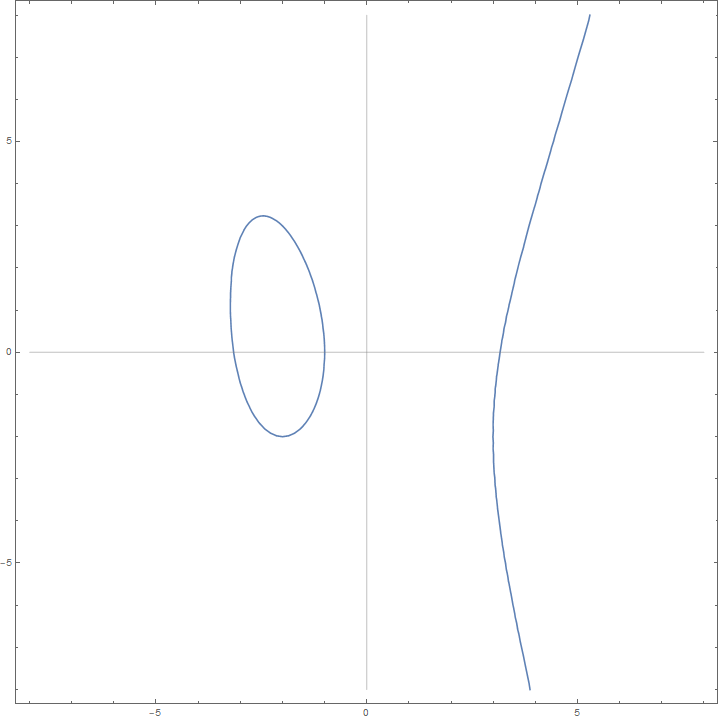
\includegraphics[scale=0.3]{figuras/eq_weierstrass}
  \caption{La curva real definida por la ecuación $Y^2+XY+Y=X^3+X^2-10X-10$.}
  \label{fig:eq_weierstrass}
\end{figure}%%%%%%%%%%%%%%%%%%%%%%%%%%%%%%%%%%%%%%%%%%%%%%%%%%%%%%%%%%%%%%%%%%%%%%%%%%%%%%%%%%%%%%%% 

\begin{nota}
Lo que hizo Fricke para calcular una ecuación de $X_0(15)$ fue un poco distinto. Él definió el $\eta-$cociente
\begin{equation}\label{eq:def_x_fricke}
	x(z):=
	\frac{\eta(3z)^3\eta(5z)^3}{\eta(z)^3\eta(15z)^3}=
	q^{-2}+3+9q^2+O(q^4).
\end{equation}
Una vez definida $x$, Fricke considera un múltiplo adecuado de la derivada de $x$ y lo llama $y$. De esta manera obtiene el segundo generador de $\CC(X_0(15))$ como $\CC-$álgebra, es decir $K(X_0(15))=\CC(x,y)$. Después, Fricke calcula y compara coeficientes de Fourier para encontrar la relación algebraica entre $x$ y $y$ que resulta ser:
\begin{equation}\label{eq:formula_fricke}
		y^2=x^4-10x^3-13x^2+10x+1.
\end{equation}
Véase \cite[página 439]{Fricke}. Es posible llevar \eqref{eq:formula_fricke} a una ecuación de Weierstrass mediante el siguiente cambio de variable:
	\[
		x\mapsto \frac{2y+x+46}{2(x-8)}+\frac{5}{2},\quad
		y\mapsto \frac{(2y+x+46)^2}{4(x-8)^2}-2(x-8)-\frac{101}{4}
	\]
De esta manera obtenemos la ecuación de Weierstrass:
	\begin{equation}\label{eq:relacionweierstrass}
		y^2+xy+y=x^3+x^2-10x-10.
	\end{equation}
\end{nota}

Con la ecuación de Weierstrass de $X_0(15)$ podemos calcular sus puntos racionales que denotamos por $G=X_0(15)(\QQ)$. Para esto usamos el teorema de Mordell-Weil\footnote{Para toda curva elíptica $E$ sobre un campo numérico $K$, el grupo $E(K)$ es un grupo abeliano finitamente generado (cf. teorema 6.7 del capítulo VIII de \cite{SilvermanTAOEC}).} que nos dice que
\[
	G\cong G_{\mathrm{tor}}\times\ZZ^r,
\]
donde $G_{\mathrm{tor}}$ es el subgrupo de torsión y $r\geq0$ es el rango de $G$. Con esta descripción de $G$, nuestra tarea se divide en dos: estudiar el grupo de torsión y calcular el rango. Primero calculamos el subgrupo de torsión con el teorema de Lutz-Nagell:\footnote{Aquí enunciamos la versión que aparece en VIII.7.2 de \cite{SilvermanTAOEC}, pero este teorema fue probado independientemente por T. Nagell y E. Lutz en los 1930's. La prueba primero apareció en \cite{Nagell} y después en \cite{Lutz}.}

\begin{thm}(Lutz-Nagell)\label{thm:Lutz-Nagelll}
	Sea $E/\QQ$ una curva elíptica con ecuación de Weierstrass
	\begin{equation}\label{eq:weierstrass-simple}
		y^2=x^3+Ax+B,\quad A,B\in\ZZ.
	\end{equation}
A la ecuación de Weierstrass le asociamos el entero $D:=4A^3+27B^2$, además denotamos $G=E(\QQ)$ y escribimos $x(P)$ y $y(P)$ como las coordenadas de $P\in G$ dadas por \eqref{eq:weierstrass-simple}. Entonces para todo $P\in G_{\mathrm{tor}}$ tenemos que $x(P),y(P)\in\ZZ$ y
\[
	P+P=O\quad\acute{o}\quad y(P)^2\mid D.
\]
\end{thm}

Este teorema lo usamos para probar:

\begin{prop}\label{prop:grupo-torsion-x15}
	Sea $G=X_0(15)(\QQ)$ el grupo de puntos racionales de la curva modular $X_0(15)$. Entonces $G_\mathrm{tor}$ tiene 8 elementos y son:
	\[
		G_\mathrm{tors}=
		\left\{ \left(-\tfrac{13}{4},\tfrac{9}{8}\right),(-1,0),(3,-2),(8,-27),(8,18),(-2,-2),(-2,3) \right\}\cup\{O\}.
	\]
\end{prop}

\begin{proof}
Para aplicar Lutz-Nagell, necesitamos transformar la ecuación de Weierstrass generalizada de $X_0(15)$ dada por el lema \ref{lema:eqweierstrassX_0(15)} a una ecuación simplificada. El cambio de variable es:
\begin{equation}\label{eq:cambio-coord-x15}
	x=\frac{x'}{36}-\frac{15}{36},\qquad y=\frac{y'}{216}-\frac{x'}{72}-\frac{21}{72}
\end{equation}
y simplifica la ecuación a
\begin{equation}\label{eq:weierstrass-simple-x15}
	y'^2=x'^3-12987x'-263466=(x'+102)(x'+21)(x'-123)
\end{equation}
donde:
\[
	D=4(-12987)^3+27(-263466)^2=-(2^4 3^8 5^2)^2.
\]

Ahora sea $P_0=(x_0,y_0)\in G_\mathrm{tor}$ donde las coordenadas están dadas por \eqref{eq:weierstrass-simple-x15}. Por Lutz-Nagell tenemos que $x_0,y_0\in\ZZ$ y el punto $P_0$ cumple una de dos casos:
\begin{enumerate}
	\item[Caso 1:] $P_0+P_0=O$.
	
	En este caso, $P_0=-P_0$. Por la ecuaci\'on \eqref{eq:coord-inverso-P}, tenemos $-P_0=(x_0,-y_0)$. Por lo tanto $P_0=-P_0$ si y solo si $y_0=0$. Ahora sustituimos $y_0=0$ en \eqref{eq:weierstrass-simple-x15} y obtenemos tres posibles valores para $x_0$ que corresponden a los siguientes tres puntos racionales de orden 2 en $G_\mathrm{tor}$:
\[
	(-102,0),\quad (-21,0)\quad\text{y}\quad (123,0)
\]
	\item[Caso 2:] $y(P_0)^2\mid D$.
	
	Si $P_0=(x_0,y_0)$, entonces por la factorización de $D$, solamente tenemos que considerar coordenadas $y_0$ que sean divisores de $2^4 3^8 5^2=\sqrt{-D}$. Sustituimos cada divisor en \eqref{eq:weierstrass-simple-x15} y resolvemos la ecuación cúbica en $x$ para obtener (o probar que no tienen) soluciones y así posibles coordenadas de $P_0$. Como $\sqrt{-D}$ tiene 270 divisores (positivos y negativos), este proceso lo verificamos con Mathematica y otenemos los siguientes cuatro puntos racionales:
	\[
		(303,4860),\quad (303,-4860),\quad (-57,-540)\quad\text{y}\quad (-57,540)
	\]
\end{enumerate}

Juntando ambos casos obtenemos la lista completa de puntos racionales de orden finito de la ecuación \eqref{eq:weierstrass-simple-x15}:
\[
	\{(-102,0),(-21,0),(123,0),(303,-4860),(303,4860),(-57,-540),(-57,540)\}\cup\{O\}.
\]
Bajo el cambio de coordenadas inverso a \eqref{eq:cambio-coord-x15}, dado por:
\[
	x'=36x+15,\quad y'=216y+108x+108
\]
podemos concluir que:
	\[
		G_\mathrm{tors}=
		\left\{ \left(-\tfrac{13}{4},\tfrac{9}{8}\right),(-1,0),(3,-2),(8,-27),(8,18),(-2,-2),(-2,3) \right\}\cup\{O\}.
	\]
\end{proof}

Como $G_\mathrm{tor}$ es abeliano y de orden 8, el teorema de estructura de grupos abelianos finitamente generados\footnote{•} nos dice que $G_\mathrm{tor}$ es isomorfo a  uno de los siguientes tres posibilidades:
\[
	\ZZ/8\ZZ\ZZ,\quad,\ZZ/2\ZZ\times\ZZ/4\ZZ,\quad\text{ó}\quad \ZZ/2\ZZ\times\ZZ/2\ZZ\times\ZZ/2\ZZ.
\]
Para saber cual de estas tres posibilidades es la correcta, necesitamos estudiar el orden del los puntos de $G_\mathrm{tor}$. Por suerte, la definición geométrica, nos permite calcular a vista la duplicación de los puntos de $G_\mathrm{tor}$.

En el diagrama \ref{fig:orden-puntos-racionales} graficamos los 7 puntos racionales afines sobre la curva elíptica y trazamos rectas tangentes en esos puntos. Si la recta tangente es vertical, omitimos la recta y marcamos el punto de verde; estos puntos son de orden 2. Si duplicamos el resto de los cuatro puntos, obtenemos el punto $(3,-2)$ que es de orden 2. Por lo tanto el resto de los puntos, i.e. $\{-2,3),(-2,-2),(8,18),(8,-27)\}$ tienen orden 4. En conclusión $G_\mathrm{tor}$ tiene tres elementos de orden 2 y cuatro de orden cuatro. Es implica que
\[
	G_\mathrm{tor}\cong\ZZ/2\ZZ\times\ZZ/4\ZZ.
\]

\begin{figure}[!h]%%%%%%%%%%%%%%%%%%%%%%%%%%%%%%%%%%%%%%%%%%%%%%%%%%%%%%%%%%%%%%%%%%%%%%%%%%% FIGURA
  \centering
  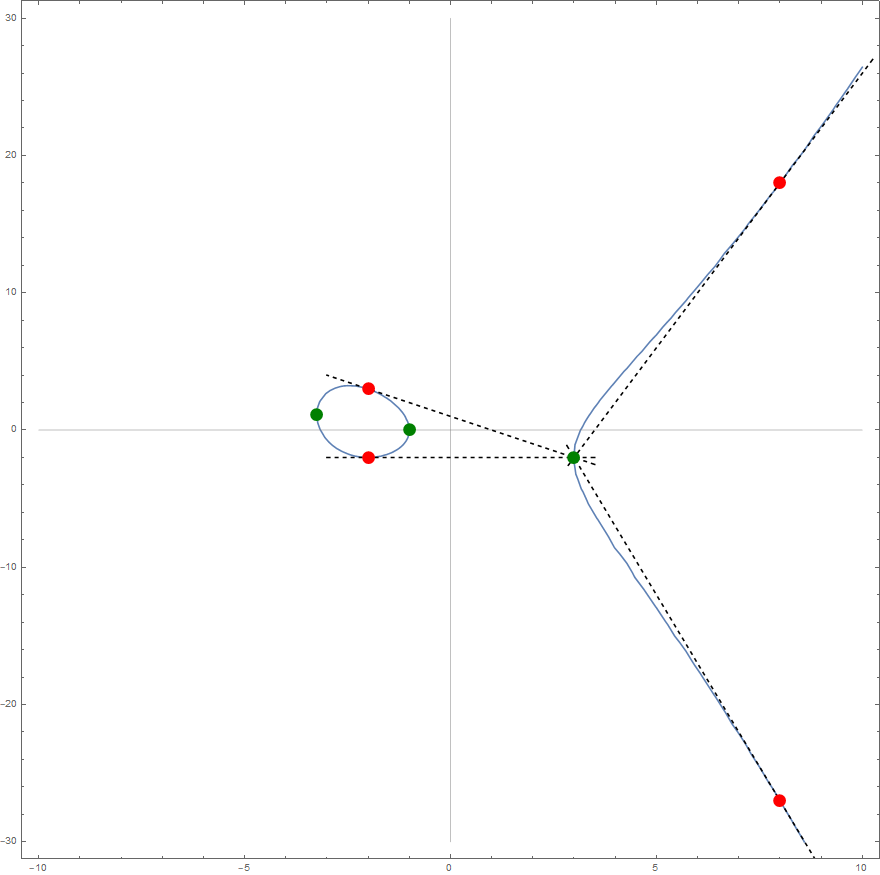
\includegraphics[scale=0.3]{figuras/orden-puntos-racionales}
  \caption{Visualización de la suplicación de los puntos racionales de $X_0(15)$. Los puntos verdes son de orden 2 y los puntos rojos son de orden 4.}
  \label{fig:orden-puntos-racionales}
\end{figure}%%%%%%%%%%%%%%%%%%%%%%%%%%%%%%%%%%%%%%%%%%%%%%%%%%%%%%%%%%%%%%%%%%%%%%%%%%%%%%%%%%%%%%%% 


Para cada punto $P\in G_\mathrm{tor}$ de orden 2, i.e. $P\in\{(-\tfrac{13}{4},\tfrac{9}{8})=,(-1,0),(3,-2)\}$, el subgrupo generado por $P$ actúa sobre $G_\mathrm{tor}$ mediante traslación:
\[
	\gen{P}\act G_\mathrm{tor}\quad\text{definido por}\quad (O,Q)\mapsto Q,\;\; (P,Q)\mapsto P+Q.
\]
Como $\gen{P}$ solamente tiene dos elementos y $G_\mathrm{tor}$ tiene ocho elementos, entonces cada acción $\gen{P}\act G_\mathrm{tor}$ descompone $G_\mathrm{tor}$ en cuatro órbitas. En la figura \ref{fig:orbitas-puntos} ilustramos estas particiones para cada punto de orden 2. Esos diagramas también muestran parte de la tabla de operaciones. En la figura \ref{fig:orbitas-puntos} vemos las órbitas de $G$ bajo la acción ${O,P}\act G$ donde $P$ corre sobre los puntos de orden 2, i.e. $P\in\{-\tfrac{13}{4},\tfrac{9}{8},(-1,0),(3,-2)\}$.

\begin{figure}\centering
\begin{minipage}[t]{0.3\textwidth}
	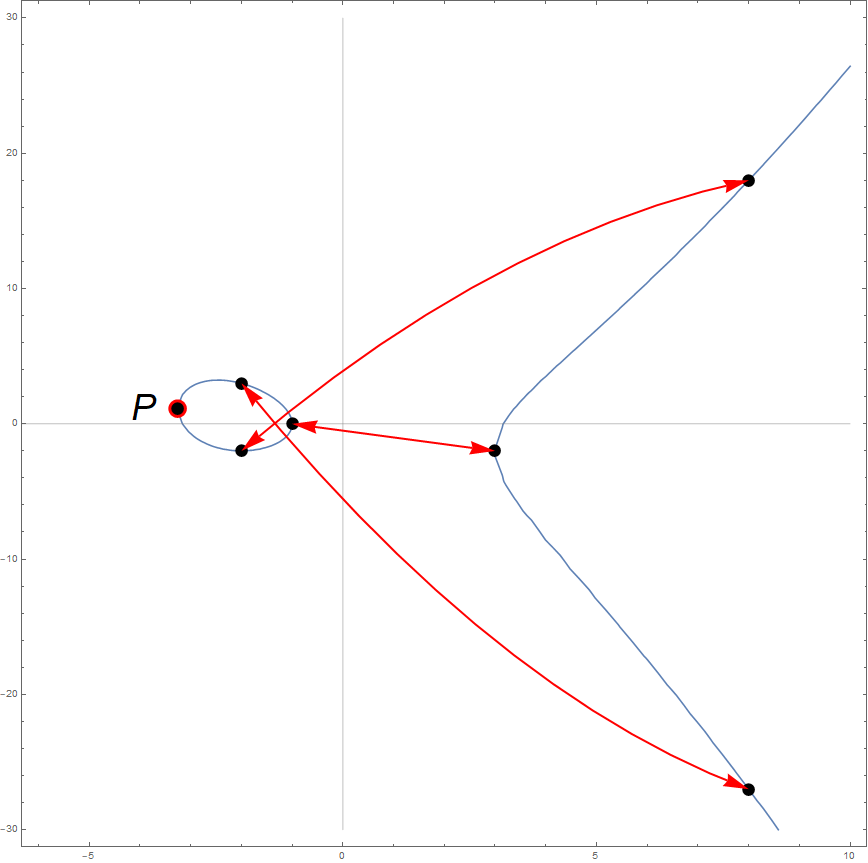
\includegraphics[width=\textwidth]{figuras/orbitas-puntos-2}
\end{minipage}
\begin{minipage}[t]{0.3\textwidth}
	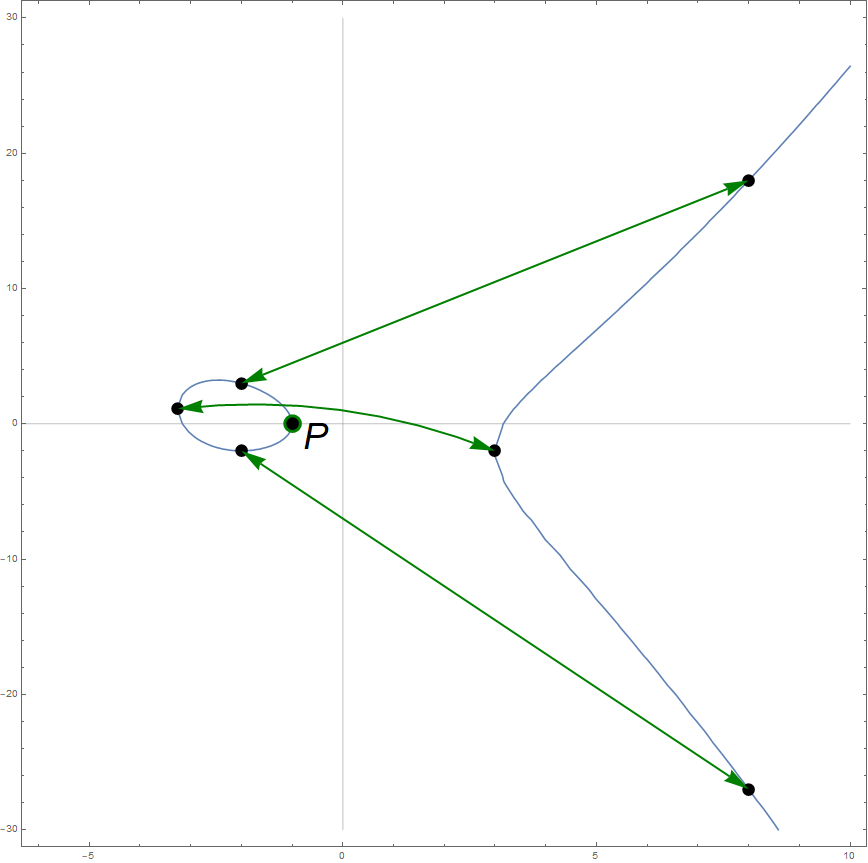
\includegraphics[width=\textwidth]{figuras/orbitas-puntos-1}
\end{minipage}
\begin{minipage}[t]{0.3\textwidth}
	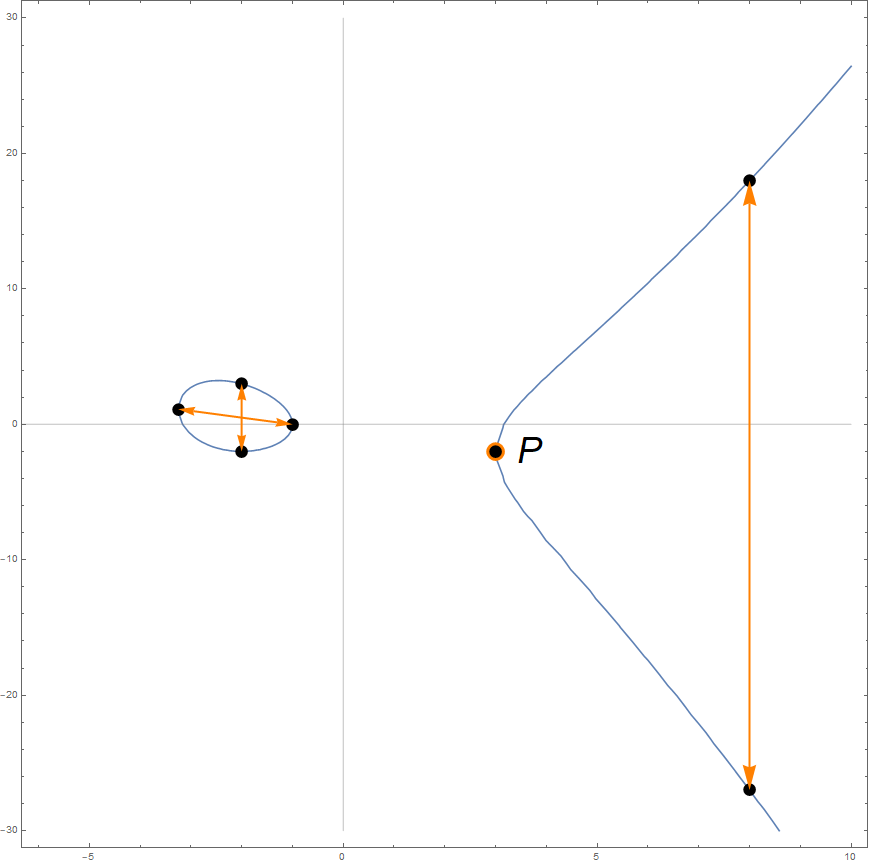
\includegraphics[width=\textwidth]{figuras/orbitas-puntos-3}
\end{minipage}
\caption{Las flechas indican la operación $+P$ donde $P$ es alguno de los tres puntos de orden 2 que tiene $X_0(15)(\QQ)$}
\label{fig:orbitas-puntos}
\end{figure}


El próximo paso es probar que el rango de $G\cong G_\mathrm{tor}\times\ZZ^r$ es cero, i.e. $r=0$. Para esto estudiamos el grupo $G/2G$ para encontrar una fórmula para $r$. El teorema de Mordell-Weil dice que $G$ es un grupo abeliano finitamente generado y por lo tanto el teorema de estructura de grupos abelianos finitamente generados nos dice que:
\[
	G\cong\ZZ^r\times\frac{\ZZ}{p_1^{n_1}\ZZ}\times\cdots\times\frac{\ZZ}{p_s^{n_s}\ZZ},
\]
para algunos números primos $p_1,\ldots,p_s\in\ZZ$ y exponentes $n_i>0$. Con esta expresión para $G$ podemos calcular $G/2G$. En efecto, tenemos que
\[
	\frac{G}{2G}\cong\left(\frac{\ZZ}{2\ZZ}\right)^r\times\frac{\ZZ/p_1^{n_1}\ZZ}{2\ZZ/p_1^{n_1}\ZZ}\times\cdots\times\frac{\ZZ/p_s^{n_s}\ZZ}{2\ZZ/p_s^{n_s}\ZZ},
\]
donde
\[
	\frac{\ZZ/p_i^{n_i}\ZZ}{2\ZZ/p_i^{n_i}\ZZ}\cong
	\begin{cases}
	\ZZ/2\ZZ & p_i=2\\
	0 & p_i\neq 2
	\end{cases}.
\]
Por lo tanto $G/2G$ es un producto de $\ZZ/2\ZZ$'s. Hay $r$ copias en la parte libre de torsión y tantas copias como potencias de 2 que aparecen en la parte de torsión, i.e.
\begin{equation}\label{eq:indice-G-2G-inicial}
	(G:2G)=2^{r+\#\{j\mid p_j=2\}}.
\end{equation}

Para calcular $2^{\#\{j\mid p_j=2\}}$, simplemente calculamos el núcleo del homomorfismo $[2]:G\ra G$ definido por $P\mapsto P+P$; al núcleo lo denotamos por $G_2$. Si $P\in G$ es de la forma $P=m_1 P_1+\cdots+m_r P_r+l_1Q_1+\cdots 1_s Q_s$ con $m_i\in\ZZ$ y $0\leq l_j<p_j^{n_j}$, entonces
\begin{align*}
	P+P=O&\quad\iff\quad 2m_1 P_1+\cdots+2m_r P_r+2l_1Q_1+\cdots 2l_s Q_s=0\\
&m_i=0,\quad 2l_j\equiv0\Mod{p_j^{n_j}}\quad\forall i,j	
\end{align*}
Si $p_j\neq2$, entonces $2$ es invertible en $\ZZ/p_j^{n_j}\ZZ$ y por lo tanto $2l_j\equiv0\Mod{p_j^{n_j}}$ es equivalente a que $l_j\equiv0\Mod{p_j^{n_j}}$. Esto junto con los posibles valores de $l_j$ implican que $l_j=0$ cuando $p_j\neq2$. Por lo tanto los únicos coeficientes de $P$ libres son las $l_j$'s tales que $p_j=2$. En este caso los únicos dos valores son $l_j=0$ ó $l_j=2^{n_j-1}$. Por lo tanto:
\[
	P+P=0\quad\iff\quad m_i=0\quad\forall i,\quad l_j=0\quad\forall j\;\text{tal que}\; p_j\neq2, \quad l_j\in\{0,2^{n_j-1}\}\quad\forall j\;\text{tal que}\; p_j=2.
\]
De esta manera el núcleo $G_2$ tiene $2^{\#\{j\mid p_j=2\}}$ elementos y por lo tanto \eqref{eq:indice-G-2G-inicial} se convierte en
\begin{equation}\label{eq:indice-G-2G}
	2^r =\frac{(G:2G)}{\# G_2}.
\end{equation}

Para calcular $r$ de la ecuación anterior, necesitamos estudiar con mayor detalle el homomorfismo $[2]:G\ra G$. La clave es decomponer $[2]$ como composición de dos homomorfismos $\varphi:G\ra \bar{G}$ y $\psi:\bar{G}\ra G$, donde $\bar{G}$ es un grupo auxiliar. Estos homomorfismos vienen de isogenias entre curvas elípticas, en particular de $X_0(15)$. Para facilitar los cálculos nos restringimos a curvas elípticas con un punto de orden 2 trasladado al origen; por suerte $X_0(15)$ tiene puntos de orden 2.

En general, sea $E$ una curva elíptica sobre $\QQ$ definida por una ecuación de la forma
\[
	E\; :\; y^2=x^3+ax^2+bx,
\]
donde $a,b\in\ZZ$ y cuyo grupo de puntos racionales denotamos por $G=E(\QQ)$. El neutro lo denotamos por $O$ y al origen lo denotamos por $T=(0,0)$; $T$ es un punto de orden 2. Por el caso 1 de la prueba de la proposición \ref{prop:grupo-torsion-x15} los puntos de orden 2 son $O$ y los puntos de la forma $P=(x,0)$. Como las coordenadas de $P$ tienen que satisfacer la ecuación de $E$, tenemos que
\[
	0=x^3+ax^2+bx=x(x^2+ax+b).
\]
Por lo tanto $a^2-4b$, el discriminante de la ecuación cuadrática $x^2+ax+b=0$, es un cuadrado perfecto si y sólo si las soluciones $x_1$ y $x_2$ de $x^2+ax+b=0$ son racionales. De esta manera tenemos que si $a^2-4b$ es un cuadrado perfecto, hay 4 puntos racionales de orden 2, i.e. $G_2=\{O,T,(x_1,0),(x_2,0)\}$ y cuando $a^2-4b$ no es un cuadrado perfecto, $(x_1,0),(x_2,0)\not\in G$ y por lo tanto solamente hay 2 puntos racionales de orden 2. Resumimos este hecho en la siguiente fórmula:
\begin{equation}\label{eq:cantidad-G2}
	\# G_2=	\begin{cases}
		4 & a^2-4b\;\text{es un cuadrado perfecto}\\
		2 & a^2-4b\;\text{no es un cuadrado perfecto}
	\end{cases}.
\end{equation}
Por lo tanto ya calculamos el término $\# G_2$ de \eqref{eq:indice-G-2G}. Ahora nos falta calcular $(G:2G)$. Para esto descomponemos el homomorfismo $[2]:G\ra G$ como composición de otros dos homomorfismos, pero primero necesitamos construir una curva elíptica auxiliar asociada a $E$.

Para toda $E$ podemos construir una curva elíptica $\bar{E}$ sobre $\QQ$ definida por:
\[
	\bar{E}\,:\, y^2=x^3+\bar{a}x^2+\bar{b}x,\quad\text{donde}\quad \bar{a}:=-2a,\;\;\bar{b}:=a^2-4b.
\]
Denotamos por $\bar{G}$ al grupo de puntos racionales de $\bar{E}$ y también denotamos por $\bar{O}$ al neutro de $\bar{E}$ y $\bar{T}$ al punto $(0,0)$ de $\bar{E}$. Observe que $\bar{b}$ es el discriminante de la ecuación cuadrática $x^2+ax+b=0$ y por lo tanto la fórmula \eqref{eq:cantidad-G2} se puede reescribir según si $\bar{b}$ es cuadrado perfecto o no.

Observe que si repetimos dos veces esta construcción obtenemos la curva $\bar{\bar{E}}$ definida por la ecuación $y^2=x^3+4ax^2+16bx$ que, bajo el cambio de variable admisible $x'=4x$ y $y'=8y$ obtenemos la ecuación original de $E$. Es decir $\bar{\bar{E}}\cong E$. 

Ahora consideramos la siguiente función: $\varphi:E\ra \bar{E}$ definido por:
\[
	\varphi(x,y):=\begin{cases}
		\paren{\tfrac{y^2}{x^2},y\tfrac{x^2-b}{x^2}} & (x,y)\neq O,T\\
		\bar{O} & (x,y)=O,T.
	\end{cases}
\]
Si aplicamos $\varphi$ a $\bar{E}$ obtenemos una función $\bar{E}\ra\bar{\bar{E}}$ que bajo el isomorfismo $\bar{\bar{E}}\cong E$, obtenemos la función $\psi:\bar{E}\ra E$ definida por
\[
	\psi(\bar{x},\bar{y}):=\begin{cases}
		\paren{\tfrac{\bar{x}^2}{\bar{y}^2},\bar{y}\tfrac{\bar{x}^2-\bar{b}}{\bar{x}^2}} & (\bar{x},\bar{y})\neq \bar{O},\bar{T}\\
		O & (\bar{x},\bar{y})=\bar{O},\bar{T}.
	\end{cases}
\]
Las funciones $\varphi$ y $\psi$ son muy útiles para estudiar la isogenia $[2]:E\ra E$ ya que cumplen las siguientes propiedades:

\begin{prop}\label{prop:descomponer-2}
	Las funciones $\varphi$ y $\psi$ definidas arriba cumplen las siguientes propiedades:
	\begin{enumerate}[label=(\roman*)]
		\item $\varphi$ y $\psi$ están bien definidas e inducen homomorfismos de grupos $\varphi:G\ra \bar{G}$ y $\psi:\bar{G}\ra G$ con núcleos $\{O,T\}$ y $\{\bar{O},\bar{T}\}$ respectivamente.
		\item\label{in:mult2} La composición de los dos homomorfismos es la multiplicación por 2, i.e. $\psi(\varphi(P))=[2]P$ para todo $P\in G$ y $\varphi(\psi(\bar{P}))=[2]\bar{P}$ para todo $\bar{P}\in\bar{G}$. Si abusamos de notación, esto lo denotamos por $$\psi\circ\varphi=[2]=\varphi\circ\psi.$$
		\item\label{in:0imagen} $\bar{O}\in\varphi(G)$ y $O\in\psi(\bar{G})$.
		\item\label{in:imagenTbar} $\bar{T}\in\varphi(G)$ (resp. $T\in\psi(\bar{G})$) si y solo si $\bar{b}$ (resp. $b$) es un cuadrado perfecto.
		\item\label{in:imagen} Si $\bar{P}=(\bar{x},\bar{y})\in\bar{G}$ con $\bar{x}\neq0$ (resp. $P=(x,y)\in G$, $x\neq0$), entonces
		\[
			\bar{P}\in\varphi(G)\;\;\big(\mathrm{resp}.\;\; P\in\psi(\bar{G})\big)\quad\iff\quad\bar{x}\in\QQ^2\;\;\big(\mathrm{resp}.\;\; x\in\QQ^2 \big).
		\]
	\end{enumerate}
\end{prop}
\begin{proof}
		Véase la proposición 3.7 de \cite{SilvermanTateRPOEC} para ver que $\varphi$ y $\psi$ están bien definidas y que cumplen (\emph{i}) y (\emph{ii}). Véase $\S3.5$ de \cite{SilvermanTateRPOEC} para la prueba de los otros dos incisos.
\end{proof}

Observe que el inciso \ref{in:mult2} garantiza que $2G=\psi(\varphi(G))\subseteq\psi(\bar{G})\subseteq G$. Por lo tanto tenemos que
\[
	(G:2G)=(G:\psi(\bar{G}))(\psi(\bar{G}):2G).
\]
Además, tenemos que\footnote{Estamos usando el siguiente resultado general de teoría de grupos abelianos: Si $f:G\ra G'$ es un homomorfismo de grupos abelianos y $H\subseteq G$ un subgrupo de índice finito, entonces
\[
	(f(G):f(H))=\frac{(G:H)}{(\ker f:H\cap\ker f)}.
\]
Esto se sigue de los teoremas de isomorfismo que nos dan:
\[
	\frac{f(G)}{f(H)}\cong\frac{G/\ker f}{H/H\cap\ker f}\cong\frac{G}{H+\ker f}\cong\frac{G/H}{(H+\ker f)/H}\cong\frac{G/H}{\ker f/(H\cap\ker f)}.
\]
En el texto usamos $G=\bar{G}$, $f=\psi$ y $H=\varphi(G)$.}
\[
	(\psi(\bar{G}):2G)=\big(\psi(\bar{G}):\psi(\varphi(G))\big)=\frac{(\bar{G}:\varphi(G))}{(\ker\psi:\varphi(G)\cap\ker\psi)}.
\]
Por lo tanto la fórmula \eqref{eq:indice-G-2G} para el rango se convierte en:
\[
	2^r=\frac{(G:\psi(\bar{G}))(\bar{G}:\varphi(G))}{(\ker\psi:\varphi(G)\cap\ker\psi)\cdot\# G_2}
\]

Primero calculamos $(\ker\psi:\varphi(G)\cap\ker\psi)$. Como $\ker\psi=\{\bar{O},\bar{T}\}$, hay solamente dos posibles valores para $(\ker\psi:\varphi(G)\cap\ker\psi)$: si $\bar{T}\in\varphi(G)$, entonces $\varphi(G)\cap\ker\psi=\ker\psi$ y as\'i $(\ker\psi:\varphi(G)\cap\ker\psi)=1$; si $\bar{T}\not\in\varphi(G)$ tenemos que $\varphi(G)\cap\ker\psi=\{O\}$ y así $(\ker\psi:\varphi(G)\cap\ker\psi)=\#\ker\psi=2$. Si juntamos estas observaciones con el inciso \ref{in:imagenTbar}, obtenemos la siguiente fórmula:
\[
	(\ker\psi:\varphi(G)\cap\ker\psi)=
	\begin{cases}
		1 & \bar{b}\;\text{es un cuadrado perfecto}\\
		2 & \bar{b}\;\text{no es un cuadrado perfecto}
	\end{cases}.
\]
Esta fórmula es afortunada porque al multiplicar $(\ker\psi:\varphi(G)\cap\ker\psi)$ por la fórmula \eqref{eq:cantidad-G2} para $\# G_2$ obtenemos $(\ker\psi:\varphi(G)\cap\ker\psi)\cdot\# G_2=4$ y por lo tanto:
\begin{equation}\label{eq:rango-indices-2}
2^{r+2}=(G:\psi(\bar{G}))(\bar{G}:\varphi(G))
\end{equation}
y el problema de calcular el rango se reduce a estudiar las imágenes de $\varphi$ y $\psi$.

Para esto recurrimos a una función puramente aritmética: consideramos $\QQ^*$ como grupo multiplicativo y tomamos el cociente con su subgrupo de cuadrados $\QQ^{*2}$, con esto definimos:
\[
	\alpha:G\lra\QQ^*/\QQ^{*2}\quad\text{con}\quad \alpha(P)=
	\begin{cases}
		x(P) \Mod{\QQ^{*2}} & x(P)\neq0\\
		1 \Mod{\QQ^{*2}} & P=O\\
		b \Mod{\QQ^{*2}} & P=T
	\end{cases}.
\]
De manera análoga, podemos definir $\bar{\alpha}:\bar{G}\ra\QQ^*/\QQ^{*2}$; simplemente hay que agregar ``-'' en donde sea necesario.

\begin{lema}
	Sea $G$ el grupo de puntos racionales de una curva elíptica $E/\QQ$. Las funciones $\alpha:G\ra\QQ^*/\QQ^{*2}$ y $\bar{\alpha}:\bar{G}\ra\QQ^*/\QQ^{*2}$ son homomorfismos de grupos y además:
	\[
		\ker\alpha=\psi(\bar{G}),\qquad \ker\bar{\alpha}=\varphi(G).
	\]
	En particular tenemos que
	\[
		(G:\psi(\bar{G}))=\#\alpha(G),\qquad (\bar{G}:\varphi(G))=\#\bar{\alpha}(\bar{G}),
	\]
	y por lo tanto, si $r$ es el rango de $E$, tenemos:
	\[
		2^{2+r}=\#\alpha(G)\cdot \#\bar{\alpha}(\bar{G}).
	\]
\end{lema}

\begin{proof}
Solamente consideramos $\alpha$ y observamos que la misma prueba funciona para $\bar{\alpha}$. Para probar que $\alpha$ es un homomorfismo de grupos, recordemos que en la sección \ref{sec:preliminares_curvas} deducimos varias ecuaciones que deben cumplir las coordenadas de $P$, $Q$ y $P+Q$. En particular la ecuación \ref{eq:prod-coord-P+Q} nos dice que:
\[
	x(P)x(Q)x(P+Q)=\mu^2,\qquad \mu=y(P)-\frac{y(Q)-y(P)}{x(Q)-x(P)}x(P)\in\QQ,
\]
o en particular
\[
	x(P)x(Q)x(P+Q)\equiv 1\Mod{\QQ^{*2}}.
\]
Si multiplicamos ambos lados de la congruencia por $x(P)x(Q)$ entonces obtenemos
\[
	x(P+Q)\equiv x(P)x(Q)\Mod{\QQ^{*2}},
\]
porque $x(P)^2\equiv x(Q)^2\equiv1\Mod{\QQ^{*2}}$ ya que $x(P),x(Q)\in\QQ$. Salvo algunos pocos casos, como cuando $Q=T$, hemos probado que $\alpha$ es un homomorfismo de grupos; el resto de los casos se siguen de la definición de $\alpha$. 

Ahora probamos que el núcleo de $\alpha$ es la imagen de $\psi$. Primero sea $P\in\ker\alpha$. Si $P=O$, por el inciso \ref{in:0imagen} de la proposición \ref{prop:descomponer-2}, tenemos que $P\in\psi(\bar{G})$. Si $b\in\QQ^{*2}$ entonces puede suceder que $P=T$, pero el inciso \ref{in:imagenTbar} nos dice que si $b$ es un cuadrado perfecto, entonces $P=T\in\psi(\bar{G})$. Por último si $P\neq O,T$, entonces
\[
	P\in\ker\alpha\quad\iff\quad x(P)\equiv 1\Mod{\QQ^{*2}} \quad\iff\quad x(P)\in\QQ^{*2} \quad\overset{*}{\iff}\quad P\in\psi(\bar{G}),
\]
donde (*) es exactamente el inciso \ref{in:imagen}. Con esto concluimos que $\ker\alpha=\psi(\bar{G})$. Las siguientes dos afirmaciones del lema se siguen del primer teorema de isomorfismo y de la fórmula \eqref{eq:rango-indices-2} para el rango que deducimos arriba. 
\end{proof}

Con este lema, hemos reducido el problema de calcular el rango de la curva elíptica $X_0(15)$, a calcular la imagen de $\alpha$ y $\bar{\alpha}$. Para hacer esto, vamos a deducir una condición necesaria que cumplen los elementos de la imagen de $\alpha$. Esto nos va a producir una lista de posibles candidatos y por lo tanto un algoritmo para calcular puntos en la imagen.

En general sea $\alpha(P)\in\alpha(G)$ donde $P=(x(P),y(P))\in G$. Si $x=0$, entonces $y(P)^2=0(0^2+a0+b)=0$ y así $P=T$. Entonces $\alpha(T)=b\QQ^{*2}\in\alpha(G)$. Si $y=0$ entonces $0=x(x^2+ax+b)$ y por lo tanto $x$ puede asumir uno de los siguientes tres valores:
\[
	x=0,\qquad x=\frac{-a\pm\sqrt{a^2-4b}}{2}=\frac{-a\pm\sqrt{\bar{b}}}{2}.
\]
Si $x=0$ nos regresamos al caso $P=T$, entonces supongamos que $x=(a\pm\sqrt{\bar{b}})/2$. Si $\bar{b}$ no es un cuadrado perfecto, entonces $x\not\in\QQ$ y por lo tanto $P\not\in G$ por lo que no obtenemos un punto nuevo en $\alpha(G)$. Si $\bar{b}$ es un cuadrado perfecto, por ejemplo $\bar{b}=d^2$, entonces
\[
	\paren{\frac{-a\pm d}{2},0}\in G\quad\then\quad \alpha\paren{\frac{-a\pm d}{2},0}=\frac{-a\pm d}{2}\QQ^{*2}.
\]
Por lo tanto los dos elementos $\tfrac{1}{2}(-a\pm d)\QQ^{*2}$ están en la imagen de $\alpha$.

El último caso $xy\neq0$ lo tratamos en el siguiente lema:

\begin{lema}\label{lema:imagen-alpha}%%%%%%%%
	Sea $G$ el grupo de puntos racionales de una curva elíptica $E$ definido por $y^2=x^3+ax^2+bx$. Para todo punto $P=(x,y)\in G$ tal que $xy\neq0$, existe un divisor $\delta$ de $b$, positivo o negativo, tal que la ecuación diofantina:
	\[
		X^2=F_\delta(Y,Z)=0,\quad\mathrm{donde}\;\mathrm{por}\quad
		F_\delta(Y,Z):=\delta Y^4+aY^2Z^2+b_0Z^4\quad(b=\delta b_0)
	\]
	tiene una solución $(X_0,Y_0,Z_0)$, con $Y_0\neq0$, y además:
	\[
		P=\left(\frac{\delta Y_0^2}{Z_0^2},\frac{\delta X_0 Y_0}{Z_0^3} \right),\qquad \alpha(P)\equiv\delta\Mod{\QQ^{*2}}.
	\]
	Si $Z_0=0$ tomamos $P=O$ y por lo tanto $\alpha(P)\equiv 1 \Mod{\QQ^{*2}}$.
\end{lema}
\begin{proof}
	Sea $P=(x,y)\in G$ tal que $x\neq0$ y $y\neq0$. Como $x,y\in\QQ$, podemos reescribir estas fracciones como
	\[
		x=\frac{m}{e^2},\qquad y=\frac{n}{e^3},
	\]
	donde $n,m,e\in\ZZ$, $e>0$ y las fracciones son irreducibles. Como $P$ es un punto sobre la curva elíptica, sus coordenadas satisfacen la ecuación que define a $E$. De esta manera tenemos:
	\[
		\paren{\frac{n}{e^3}}^2=\frac{m}{e^2}\left(\frac{m^2}{e^4}+a\frac{m}{e^2}+b\right) \quad\then\quad n^2=m(m^2+ame^2+e^4b).
	\]
	
	Por otro lado, sea $\delta=\pm(m,b)$ donde elegimos el signo de tal manera que $\delta m>0$. Con esto en mente escribimos $m=\delta m_0$ y $b=\delta b_0$ donde, por construcción, tenemos que $(m_0,b_0)=1$. Si sustituimos estas expresiones en la ecuación anterior, obtenemos:
	\begin{gather}
		n^2=\delta m_0(\delta^2m_0^2+a\delta m_0 e^2+e^4\delta b_0)=\delta^2m_0(\delta m_0^2+ae^2m_0+e^4b_0),\label{eq:diofantina-preliminar}\\
		\therefore\quad\delta^2\mid n^2\quad\then\quad \delta\mid n.\nonumber
	\end{gather}
Con esto, escribimos $n=\delta n_0$ y volvemos a sustituir en la ecuación \eqref{eq:diofantina-preliminar} para obtener:
	\begin{equation}\label{eq:diofantina-preliminar-2}
		\delta^2n_0^2=\delta^2m_0(\delta m_0^2+ae^2m_0+e^4b_0) \quad\then\quad n_0^2=m_0(\delta m_0^2+ae^2m_0+e^4b_0).
	\end{equation}
		
	El siguiente paso es probar que los dos factores de lado derecho, $m_0$ y $\delta m_0^2+ae^2m_0+e^4b_0$, son primos relativos. De esta manera tendríamos que ambos factores son cuadrados perfectos. Para esto, supongamos que existe un primo $p$ que es un factor común. Primero observemos que como $p\mid m_0$ y $(m_0,b_0)=1$, entonces $p\nmid b_0$. Además tenemos que:
	\begin{gather*}
		p\mid \delta m_0^2+ae^2m_0+e^4b_0 \quad\then\quad p\mid e^4b_0 \quad\overset{p\nmid b_0}{\then}\quad p\mid e^4 \quad\then\quad p\mid e\\
		\therefore\quad p\mid(m_0,e) \quad\then\quad p\mid (m,e)=1 \quad\ra\leftarrow.
	\end{gather*}
La contradicción es por elección de $m$ y $e$ que tomamos como primos relativos. Por lo tanto el primo $p$ no puede existir y así $m_0$ y $\delta m_0^2+ae^2m_0+e^4b_0$ son primos relativos.

Gracias a lo anterior y a \eqref{eq:diofantina-preliminar-2}, existen enteros $N$ y $M$ tales que
\[
	M^2=m_0,\qquad N^2=\delta m_0^2+ae^2m_0+e^4b_0.
\]
Con esto, \eqref{eq:diofantina-preliminar-2} implica que $n_0=MN$. Si sustituimos estas nuevas expresiones en \eqref{eq:diofantina-preliminar-2}, obtenemos:
\[
	(MN)^2=M^2(\delta M^4+ae^2M^2+e^4b_0)\quad\then\quad N^2=\delta M^4+aM^2e^2+b_0e^4.
\]
Por lo tanto  $(X,Y,Z)=(N,M,e)$ es una solución de la ecuación diofantina:
\[
	X^2=\delta Y^4+aY^2Z^2+b_0 Z^4.
\]

Además, el punto $P$ tiene coordenadas:
\[
	P=(x,y)=\paren{\frac{m}{e^2},\frac{n}{e^3}}=\paren{\delta\frac{M^2}{e^2},\frac{\delta MN}{e^3}}.
\]
Por lo tanto
\[
	\alpha(P)=\delta\frac{M^2}{e^2}\equiv \delta\Mod{\QQ^{*2}} \quad\then\quad \delta\Mod{\QQ^{*2}}\in\alpha(G).
\]
\end{proof}

Con el lema anterior nos sugiere un algoritmo que calcula la imagen de $\alpha$: toma todos los divisores de $b$ y ve si la ecuación diofantina $X^2=F_\delta(Y,Z)$ tiene solución; los que tengan solución nos producen elementos en la imagen y todos los elementos en la imagen surgen de esta manera.

Podemos mejorar el algoritmo. Supongamos que hay dos divisores $\delta_1$ y $\delta_2$ tales que $\delta_1\equiv\delta_2\Mod{\QQ^{*2}}$. Entonces existe un racional $d/e\in\QQ$ tal que $\delta_1 e^2=\delta_2 d^2$. Esto implica que el punto $P$ asociado a la solución $(X_0,Y_0,Z_0)$ es igual a:
	\[
		P=(\delta_1 Y_0^2Z_0^{-2},\delta_1 X_0Y_0Z_0^{-3})=(\delta_2 (dY_0)^2(eZ_0)^{-2},\delta_2 (deX_0)(dY_0)(eZ_0)^{-3}),
	\]
que es el punto asociado a la solución $(deX_0,dY_0,eZ_0)$ de la ecuación diofantina asociada a $\delta_2$, en efecto:
	\begin{align*}
		\delta_2(d Y_0)^4+a(d Y_0)^2(eZ_0)^2+\frac{b}{\delta_2}(eZ_0)^4
		&=\frac{e^2}{d^2}\delta_1(d Y_0)^4+a(d Y_0)^2(eZ_0)^2+\frac{b d^2}{\delta_1 e^2}(eZ_0)^4\\
		&=e^2d^2 (\delta Y_0^4+aY_0^2 Z_0^2+b_0Z_0^4)\\
		&=e^2d^2X_0^2,
	\end{align*}
	\[
		\therefore\quad (deX_0)^2=F_{\delta_2}(dY_0,eZ_0).
	\]
Acabamos de probar que si $\delta_1\equiv\delta_2\Mod{\QQ^{*2}}$ entonces $X^2=F_{\delta_1}(Y,Z)$ tiene solución si y solo si $X^2=F_{\delta_2}(Y,Z)$ tiene solución.

Por lo tanto si partimos el conjunto de divisores de $b$ en clases de equivalencia módulo $\QQ^{*2}$, entonces basta verificar si $X^2=F_\delta(Y,Z)=0$ para solamente un divisor $\delta$ por cada clase de equivalencia. De esta manera tenemos el siguiente algoritmo para calcular la imagen de $\alpha$:

\begin{alg}\label{alg:puntos-racionales}
Cálculo de $\alpha(G)$. Sea $G$ el grupo de puntos racionales de una curva elíptica $E$ definido por $y^2=x^3+ax^2+bx$. Denotamos por $\mathfrak{D}$ al conjunto de divisores positivos y negativos de $b$.
\begin{enumerate}
	\item Parte $\mathfrak{D}$ en clases de equivalencia módulo $\QQ^{*2}$ y toma un sistema completo de residuos $\mathfrak{D}'=\{\delta_1,\ldots,\delta_n\}$ módulo $\QQ^{*2}$.
	\item Para todo divisor $\delta_i\in\mathfrak{D}'$, determina si la ecuación diofantina $X^2=\delta_i Y^4+aY^2Z^2+b_i Z^4$ (donde $b=\delta_i b_i$) tiene una solución $(X_i,Y_i,Z_i)$ con $Y_i\neq0$.
	\begin{enumerate} 
		\item\label{in:existencia-diof} Si existe tal solución, entonces $b\Mod{\QQ^{*2}}\in\alpha(G)$.
		\item Si no tiene tal solución, cambia de divisor y repite.
	\end{enumerate}
	\item Cuando se terminen los divisores, la lista de elementos obtenidos en \ref{in:existencia-diof} es la imagen de $\alpha$.
\end{enumerate}
\end{alg}

\begin{nota}
	Cuando $\bar{b}$ es un cuadrado perfecto vimos que $\frac{-a\pm d}{2}\QQ^{*2}$ son dos elementos de la imagen de $\alpha$, pero el algoritmo anterior ya nos produce estos dos elementos. En efecto, si $\bar{b}=d^2$ es un cuadrado perfecto, entonces $b$ admite la factorización
	\[
		b=\frac{-a+d}{2}\frac{-a-d}{2}\QQ^{*2}.
	\]
	Si tomamos $\delta=(-a\pm d)/2$, entonces la ecuación diofantina:
	\[
		X^2=\frac{-a\pm d}{2} Y^4+aY^2Z^2+\frac{-a\mp d}{2}Z^4
	\]
	tiene la solución trivial $(X_0,Y_0,Z_0)=(0,1,1)$ y por lo tanto el algoritmo nos produce los dos elementos $\frac{-a\pm d}{2}\QQ^{*2}$.
\end{nota}

\begin{comment}%%%%%%%%%%%%%%%%%%%%%%%%%%%%%%%%%%%%%%%%%%%%%%%%%%%%%%%COMENTARIO
\begin{ejemplo} 
Aplicamos el algoritmo deducido del lema \ref{lema:imagen-alpha} a $G=X_0(15)(\QQ)$ y deducimos que
\begin{equation}\label{eq:imagen-alpha}
	\alpha(G)=\big\{1\Mod{\QQ^{*2}},-1\Mod{\QQ^{*2}}\big\}\quad\then\quad \#\alpha(G)=2.
\end{equation}
Primero tenemos que reescribir la ecuación de Weierstrass. Empezamos con la ecuación de Weierstrass simplificada \eqref{eq:weierstrass-simple-x15} que usamos para aplicar el teorema de Lutz-Nagell. Podríamos simplemente trasladar uno de los puntos de orden 2 al origen, pero la ecuación resultante tendría coeficientes muy grandes. Entonces mejor tomamos el cambio de variable:
\[
	x'=9x-21,\qquad y'=27y
\]
y la ecuación \ref{eq:weierstrass-simple-x15} se convierte en
\[
	y^2=x^3-7x^2-144x.
\]
En este caso tenemos $a=-7$, $b=-144=-2^4 3^2$.

Todo divisor $\delta$ de $b$ es de la forma $\pm 2^\alpha3^\beta$ donde $0\leq\alpha\leq4$ y $0\leq\beta\leq2$, entonces módulo $\QQ^{*2}$ tenemos que
\[
	\delta=\pm2^\alpha3^\beta\equiv
	\begin{cases}
		\pm1\Mod{\QQ^{*2}} & 2\mid\alpha,\;\; \beta=0,2\\
		\pm2\Mod{\QQ^{*2}} & 2\nmid\alpha,\;\; \beta=0,2\\
		\pm3\Mod{\QQ^{*2}} & 2\mid\alpha,\; \beta=1\\
		\pm6\Mod{\QQ^{*2}} & 2\nmid\alpha,\;\;\beta=1
	\end{cases}.
\]
Por lo tanto, $\{-6,-3,-2,-1,1,2,3,6\}$ es un sistema completo de residuos módulo $\QQ^{*2}$. En lo que sigue probaremos que para $\delta=\pm1$ las ecuaciones diofantinas asociadas tienen solución, pero para el resto de las ecuaciones diofantinas no tienen solución.
\begin{enumerate}
	\item[($\delta=1$)] $(X_0,Y_0,Z_0)=(1,1,0)$ es una solución de $X^2=Y^4-7Y^2Z^2-144Z^4$ y corresponde al punto $O$.
	
	
	\item[($\delta=-1$)] $(X_0,Y_0,Z_0)=(0,3,1)$ es una solución de $X^2=-Y^4-7Y^2Z^2+144 Z^4$ y corresponde al punto $(-9,0)$.
	
	
	\item[($\delta=\pm6$)] La ecuación diofantina $X^2=F_\delta(Y,Z)=0$ no tiene solución. El siguiente argumento es independiente del signo de $\delta$, entonces tomamos $\delta=6$. Supongamos que	tiene una solución $(X_0,Y_0,Z_0)$. Entonces:
	\begin{equation}\label{eq:divseis2}
		X_0^2=6Y_0^4-7Y_0^2 Z_0^2 -24 Z_0^4.
	\end{equation}
	Si reducimos la ecuación módulo 3, obtenemos:
	\[
		X_0^2\equiv -(Y_0Z_0)^2 \Mod{3}.
	\]
	Como $-1$ no es un residuo cuadrático módulo 3, esto solamente sucede cuando $X_0\equiv0\Mod{3}$. Escribimos $X_0=3x_0$ para algún entero $x_0$. Además $Y_0Z_0\equiv0\mod{3}$. Sin pérdida de generalidad supongamos que $Y_0\equiv0\Mod{3}$, entonces $Y_0=3y_0$ para alguna $y_0\in\ZZ$. Sustituimos esto en la ecuación diofantina \eqref{eq:divseis2} y obtenemos:
	\[
		3^2 x_0^2 = 2\cdot 3^5y_0^4- 63 y_0^2 Z_0^2 -24 Z_0^4 \quad\then\quad
		3x_0^2 = 2\cdot 3^4 y_0^4- 21 y_0^2 Z_0^2 -8 Z_0^4 \quad\then\quad 3\mid Z_0.
	\]
	Entonces, si escribimos $Z_0=3z_0$, entonces la ecuación diofantina  anterior se reescribe como:
	\begin{gather*}
		3x_0^2 = 2\cdot 3^4 y_0^4- 3^3 7 y_0^2 z_0^2 -2^3 3^4 z_0^4\quad\then\quad
		x_0^2 = 2\cdot 3^3 y_0^4- 3^2 7 y_0^2 z_0^2 -2^3 3^3 z_0^4,\\
		\therefore\quad \paren{\frac{x_0}{3}}^2= 6 y_0^4-7y_0^2 z_0^2-24z_0^4=F_6(y_0,z_0).
	\end{gather*}
	Por lo tanto si $(X_0,Y_0,Z_0)$ es una solución de $X^2=F_6(Y,Z)$, entonces $(x_0/3,y_0,z_0)$ es otra solución cuyas entradas son estrictamente menores a la solución original. Por lo tanto podemos construir una cadena infinita de soluciones enteras cuyas entradas decrecen estrictamente. Esto es un ejemplo de \emph{descenso a infinito}, un método famoso para probar que una ecuación diofantina no tiene solución. Por lo tanto $(x_0,Y_0,Z_0)$ no puede existir, es decir $X^2=F_{\pm6}(Y,Z)$ no tiene soluciones y $\delta=\pm 6$ no contribuye a la imagen de $\alpha$.

	
	
	\item[($\delta=\pm 2,3$)] Vamos a probar que la ecuación diofantina $X^2=F_\delta(Y,Z)$ no tiene solución. Una clave para hacer los cuatro casos juntos es observar que $2\equiv2^3 3^2$ y $3\equiv 2^2 3^3\Mod{\QQ^{*2}}$, es decir:
	\[
		\delta\equiv2^{\alpha}3^\beta\Mod{\QQ^{*2}},\quad\text{tales que}\quad |\alpha-\beta|=1.
	\]
Supongamos que $(X_0,Y_0,Z_0)$ es una solución a la ecuación diofantina. Los divisores -3,-2,2 y 3 son de la forma $\delta=\pm2^\alpha 3^\beta$ donde $|\alpha-\beta|=1$. Ahora reducimos la ecuación diofantina asociada a $\delta$ , módulo 5 para obtener la congruencia:
\begin{equation}\label{eq:congmod5}
	X_0^2\equiv \pm2^\alpha 3^\beta Y_0^4 -7 Y_0^2 Z_0^2 \mp 2^{4-\alpha} 3^{2-\beta} Z_0^4 \Mod{5}.
\end{equation}
Observe que $2\cdot3\equiv 1\Mod{5}$, entonces $3^{\beta}\equiv 2^{-\beta}$ y por lo tanto la congruencia anterior se reduce a
\[
	X^2\equiv \pm 2^{\alpha-\beta} Y_0^4 +2 Y_0^2 Z_0^2 \mp 2^{\beta-\alpha-2} Z_0^4 \Mod{5}.
\]

Por el pequeño teorema de Fermat, tenemos que $Y_0^4\equiv1$ ó $Y_0^4\equiv0\Mod{5}$ según si $5\nmid Y_0$ o no. Por lo tanto:
\[
	X_0^2\equiv
	\begin{cases}
	\pm 2^{\alpha-\beta}+2 Y_0^2 Z_0^2 \mp 2^{\beta-\alpha-2} \Mod{5} & Y_0,Z_0\not\equiv0\Mod{5}\\
	\mp 2^{\beta-\alpha-2} \Mod{5} & Y_0\equiv0, Z_0\not\equiv0\Mod{5}\\
	\pm 2^{\alpha-\beta} \Mod{5} & Y_0\not\equiv0, Z_0\equiv0\Mod{5}\\
	0 & Y_0\equiv Z_0\equiv0\Mod{5}
	\end{cases}.
\]
Como $-2^{-2}\equiv -4^{-1}\equiv -(-1)^{-1}\equiv 1\Mod{5}$, entonces lo anterior se reduce a
\[
	X_0^2\equiv
	\begin{cases}
	2(Y_0Z_0)^2 \pm(2^{\alpha-\beta}+2^{\beta-\alpha})\Mod{5} & Y_0,Z_0\not\equiv0\Mod{5}\\
	\pm 2^{\beta-\alpha} \Mod{5} & Y_0\equiv0, Z_0\not\equiv0\Mod{5}\\
	\pm 2^{\alpha-\beta} \Mod{5} & Y_0\not\equiv0, Z_0\equiv0\Mod{5}\\
	0 & Y_0\equiv Z_0\equiv0\Mod{5}
	\end{cases}.
\]
En este caso $|\alpha-\beta|=1$, así la suma dentro del paréntesis es igual a $2+2^{-1}\equiv2+3\equiv0\Mod{5}$. Concluimos que
\[
	X_0^2\equiv
	\begin{cases}
	2(Y_0Z_0)^2 & Y_0,Z_0\not\equiv0\Mod{5}\\
	2,3 \Mod{5} & Y_0\equiv0, Z_0\not\equiv0\Mod{5}\\
	2,3 \Mod{5} & Y_0\not\equiv0, Z_0\equiv0\Mod{5}\\
	0 & Y_0\equiv Z_0\equiv0\Mod{5}
	\end{cases}.
\]
Como 2 y 3 no son un residuos cuadráticos módulo 5, los tres primeros casos no pueden suceder. Por lo tanto $Y_0\equiv Z_0\equiv0\Mod{5}$. De la ecuación \eqref{eq:congmod5} también concluimos que $X_0\equiv 0\Mod{5}$.

Escribimos $X_0=5x_0$, $Y_0=5y_0$ y $Z_0=5z_0$, y lo sustituimos en la ecuación diofantina $X^2=F_\delta(Y,Z)$, obtenemos:
\begin{gather*}
	\paren{\frac{x_0}{5}}^2 =\pm2^\alpha 3^\beta y_0^4 -63 y_0^2 z_0^2 \mp 2^{4-\alpha}3^{2-\beta} z_0^4,\\
	\therefore\quad \paren{\frac{X_0}{25},\frac{Y_0}{5},\frac{Z_0}{5}}\;\;\text{es una solución de}\;\; X^2=F_\delta(Y,Z).
\end{gather*}
Otra vez por un argumento de descenso a infinito, vemos que una solución $(X_0,Y_0,Z_0)$ de la ecuación diofantina $X^2=F_\delta(Y,Z)0$ no puede existir.
\end{enumerate}

Con todos los casos resueltos, podemos concluir que
\[
		\alpha(G)=\{\alpha(O),\alpha(-81,0)\}=\big\{1\Mod{\QQ^{*2}},-1\Mod{\QQ^{*2}}\big\}
\]
y verificamos \eqref{eq:imagen-alpha}.
\end{ejemplo}
\end{comment}%%%%%%%%%%%%%%%%%%%%%%%%%%%%%%%%%%%%%%%%%%%%%%%%%%%%%%%%COMENTARIO


Usamos este algoritmo para probar que

\begin{prop}\label{prop:rango-X015}
  El rango de la curva modular elíptica $X_0(15)$ es 0, por lo tanto, si $G=X_0(15)(\QQ)$ es su grupo de puntos racionales, entonces $G=G_\mathrm{tor}$ y $\# G=8$.
\end{prop}

\begin{proof}
	Si aplicamos el algoritmo a la curva $X_0(15)$ con la ecuación de Weierstrass $y^2+xy+y=x^3+x^2-10x-10$, los coeficientes de las ecuaciones diofantinas son muy grandes para describir el proceso en este texto. Entonces, como el rango es invariante bajo isogenias (cf. la segunda nota después del teorema \ref{thm:kernel-isogenias}), vamos a cambiar $X_0(15)$ por una curva isógena que tenga coeficientes más pequeños. Para encontrar tal curva, primero buscamos la ecuación de Weierstrass de $X_0(15)$ en las tablas de Cremona \cite{Cremona}; está en la lista de curvas de conductor 15.\footnote{En general, cuando $X_0(N)$ es una curva elíptica, entonces su conductor es $N$; esto lo prueba Ligozat en su tesis. Además, comentamos que si usamos las tablas de Cremona, entonces a priori tenemos que el rango de $X_0(15)$ es 0, pero solamente estamos invocando las tablas de Cremona para simplificar los cálculos y la exposición.}
	
	Ahora buscamos otra curva elíptica en esa misma clase de isogenia con coeficientes más pequeños, en este caso tomamos la ecuación $y^2+xy+y= x^3+x^2$. Si simplificamos la ecuación de Weierstrass, obtenemos $y^2=x^3-27x+8694$ y después del cambio de variable $(x,y)\ra (9x-21,27y)$, obtenemos una ecuación de Weierstrass de la forma adecuada para aplicar el algoritmo \ref{alg:puntos-racionales}:
\[
	E\; : \; y^2=x^3-7x^2+16x.
\]
Las constantes necesarias para el algoritmo son $a=-7$ y $b=2^4$. De una vez calculamos la curva elíptica asociada:
\[
	\bar{E}\; :\; y^2=x^3+14x^2-15x,
\]
donde $\bar{a}=14$ y $\bar{b}=-15$. Aplicamos el el primer paso del algoritmo a $E$ y a $\bar{E}$:

Todo divisor $\delta$ de $b$ es de la forma $\pm 2^\alpha$ donde $0\leq\alpha\leq4$. Si $2\mid\alpha$, entonces $\delta$ es un cuadrado perfecto y $\pm\delta\equiv\pm1\Mod{\QQ^{*2}}$; si $2\nmid\alpha$ tenemos $\pm 2^\alpha\equiv\pm 2\Mod{\QQ^{*2}}$. Por lo tanto.
\[
	\mathfrak{D}'=\{-2,-1,1,2\}.
\]
Todos los divisores de $\bar{b}$ son libres de cuadrados, entonces ninguna pareja de divisores son congruentes módulo $\QQ^{*2}$ y por lo tanto
\[
	\bar{\mathfrak{D}}'=\mathfrak{D}=\{-15,-5,-3,-1,1,3,5,15\}.
\]

En el caso $E$, la ecuación asociada al divisor $\delta\mid b$
\[
	X^2=F_\delta(Y,Z)=\delta Y^4-7 Y^2 Z^2+\frac{16}{\delta}Z^4
\]
no tiene solución real (no trivial) cuando $\delta<0$ porque en este caso $16/\delta<0$ y así el lado derecho es negativo. Por lo tanto, si $\delta<0$, la ecuación diofantina $X^2=F_\delta(Y,Z)$ no tiene solución y por lo tanto $\delta\Mod{\QQ^{*2}}\not\in\alpha(G)$; descartamos los divisores negativos y nos quedamos con solamente $\delta=1,2$. Si $\delta=1$ tenemos que
\[
	(1,1,0)\;\;\text{es una solución de}\quad X^2=Y^4-7 Y^2 Z^2+16Z^4.
\]
Por lo tanto $1\Mod{\QQ^{*2}}\in\alpha(G)$, pero esto ya lo sabíamos porque $\alpha(O)=1\mod{\QQ^{*2}}$. Sin embargo, si $\delta=2$, la ecuación diofantina $X^2=2Y^4-7 Y^2 Z^2+8 Z^4$, no tiene soluciones.

Para ver esto reducimos la ecuación módulo 4:
\begin{equation}\label{eq:diof-mod-4}
	X_0^2\equiv 2 Y_0^4+Y^2 Z^2\equiv Y_0^2(2Y_0^2+Z_0^2) \Mod{4}.
\end{equation}
Hay dos casos según si $Y_0^2\equiv0$ ó $Y_0^2\equiv1\Mod{4}$, ya que éstos son los únicos residuos cuadráticos módulo 4. Si ocurre lo último tenemos:
\begin{equation}\label{eq:2-noRC-mod-4}
	Y_0\equiv1\Mod{4}\quad\then\quad
	X_0^2\equiv 2+Z_0^2\equiv\begin{cases}2\Mod{4} & Z_0^2\equiv0\Mod{4}\\ -1\Mod{4} & Z_0^2\equiv1\Mod{4} \end{cases}
	\quad\ra\leftarrow.
\end{equation}
Por lo tanto necesariamente tenemos $Y_0^2\equiv0\Mod{4}$ ó equivalentemente $2\mid Y_0$. Esto, junto con la congruencia \eqref{eq:diof-mod-4}, implica que $X_0^2\equiv0\Mod{4}$ y también $2\mid X_0$.

Por lo tanto existen $x_0,y_0\in\ZZ$ tales que $X_0=2x_0$ y $Y_0=2y_0$. Si sustituimos esto en la ecuación diofantina original para $\delta=2$, obtenemos:
\begin{equation}\label{eq:diof2-reducido}
	4x_0^2= 32 y_0^4-28y_0^2 Z_0^2+8Z_0^4=4(8 y_0^4-7y_0^2 Z_0^2+2Z_0^4)\quad\then\quad
	x_0^2=8 y_0^4-7y_0^2 Z_0^2+2Z_0^4.
\end{equation}
Módulo 4 la ecuación se vuelve
\[
	x_0^2\equiv Z_0^2(y_0^2+2Z_0^2).
\]
Si $Z_0^2\equiv1\Mod{4}$ obtenemos la misma contradicción que en \eqref{eq:2-noRC-mod-4}, entonces $Z_0^2\equiv0\Mod{2}$, i.e. $Z_0=2z_0$ para alguna $z_0\in\ZZ$. Esto, junto con la congruencia anterior, implica que también $x_0^2\equiv0\Mod{4}$; escribimos $x_0=2x_1$ para alguna $x_1\in\ZZ$. Sustituimos estas expresiones en la ecuación \eqref{eq:diof2-reducido} para obtener
\[
	4x_1^2=8 y_0^4-28y_0^2 z_0^2+32z_0^4\quad\then\quad
	x_1^2=2y_0^4-7y_0^2z_0^2+8z_0^4,
\]
es decir $(x_1,y_0,z_0)=(X_0/4,Y_0/2,Z_0/2)$ es una solución a la ecuación diofantina $X^2=F_2(Y,Z)$.

Observe que las entradas de la nueva solución son estrictamente menores que las entradas originales y en particular $0<Y_0/2<Y_0$. Por lo tanto podemos construir una cadena infinita de soluciones enteras cuyas entradas decrecen estrictamente, lo cual es imposible. Esto es un ejemplo de \emph{descenso a infinito}, un método famoso para probar que una ecuación diofantina no tiene solución. Por lo tanto $X^2=F_2(Y,Z)$ no tiene soluciones y de esta manera el divisor $\delta=2$ no contribuye a la imagen. Hemos probado que
\begin{equation}\label{eq:imag-alpha-G}
	\alpha(G)=\{1\Mod{\QQ^{*2}}\}\quad\then\quad \#\alpha(G)=1 
\end{equation}

Ahora estudiamos las ecuaciones diofantinas asociadas a la curva $\bar{E}$: para todo divisor $\bar{\delta}\in\bar{\mathfrak{D}}'$, la ecuación diofantina asociada a $\bar{\delta}$ es $X^2=F_{\bar{\delta}}(Y,Z)$ donde $F_{\bar{\delta}}$ está definida por
\[
	F_{\bar{\delta}}(Y,Z)=\bar{\delta}Y^4+14Y^2 Z^2-\frac{15}{\delta}Z^4.
\]

Al tanteo, uno puede encontrar soluciones pequeñas a varias ecuaciones diofantinas. Por ejemplo:
\begin{gather*}
	(0,1,1)\;\;\text{es una solución de}\quad X^2=Y^4+14 Y^2 Z^2-15Z^4\;\;\text{y}\;\; X^2=-15Y^4+14 Y^2 Z^2+1Z^4, \\
	(4,1,1)\;\;\text{es una solución de}\quad X^2=5Y^4+14 Y^2 Z^2-3Z^4\;\;\text{y}\;\; X^2=-3Y^4+14 Y^2 Z^2+5Z^4.
\end{gather*}
Entonces las ecuaciones asociadas a $\bar{\delta}=-15,-3,1,5$ tienen soluciones. Por lo tanto:
\begin{equation}\label{eq:imag-alphabar}
	\{-15\Mod{\QQ^{*2}},-3\Mod{\QQ^{*2}},1\Mod{\QQ^{*2}},5\Mod{\QQ^{*2}}\}\subseteq\bar{\alpha}(\bar{G}).
\end{equation}



El resto de las ecuaciones no tienen soluciones. Como ya hemos descrito con detalle este proceso para la curva $E$, solamente mencionamos bajo qué módulo sale la contradicción. Para $F_{-1}(Y,Z)$ y $F_{15}(Y,Z)$, reduce módulo 8 porque ahí $F_{-1}\equiv F_{15}\Mod{8}$; para $F_3(Y,Z)$ y $F_{-15}(Y,Z)$, reduce módulo 16. En ambos casos, la existencia de una solución nos produce una contradicción mediante un argumento de ``descenso a infinito''. Concluimos que la contención de \eqref{eq:imag-alphabar} es una igualdad y por lo tanto
\begin{equation}\label{eq:card-imag-alphabar}
	\#\bar{\alpha}(\bar{G})=4.
\end{equation}
Para terminar juntamos nuestras fórmulas para las imágenes de $\alpha$, (es decir \eqref{eq:imag-alpha-G} y \eqref{eq:card-imag-alphabar}), y sustituimos en la fórmula del rango de $E$ del lema \ref{lema:imagen-alpha} para concluir que:
\[
	2^{2+r}=4\quad\then\quad r=0.
\]
\end{proof}






\end{document}
